\section{Identification of wave spectrum model}
\subsection{Problem a}
The MATLAB function \texttt{pwelch} calculates an estimate of the power spectral density PSD through
dividing the signal $\psi_w$ into K overlapping blocks multiplied by a windowing function, and finding an
estimate for the periodogram of each one.

\begin{figure}[h]
    \centering
    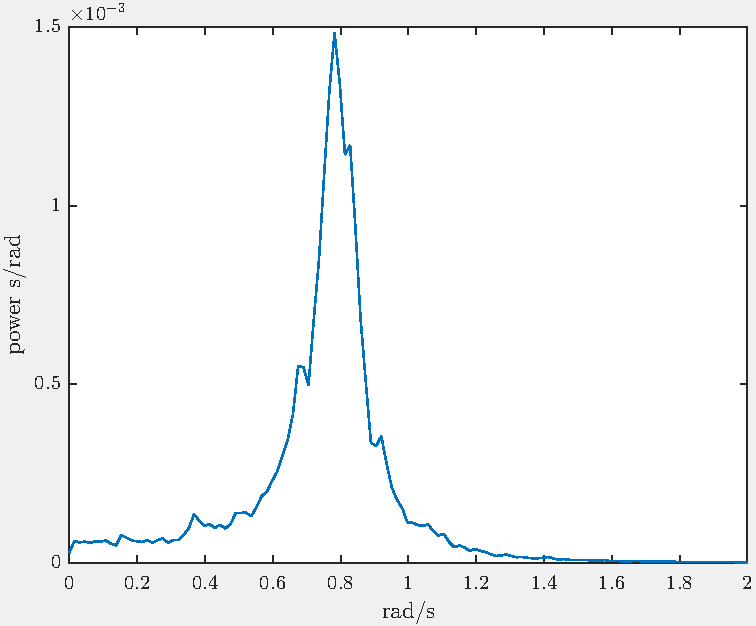
\includegraphics[width=0.5\textwidth]{images/2a-welchPSDestimate}
    \caption{Welch PSD estimate}
    \label{fig:2a-welchPSDestimate}
\end{figure}

\subsection{Problem b}
Using the following state equations in the problem description \cite{assignment}

\begin{align*}
    \xi_w &= \psi_w \\
    \dot{\psi}_w &= -\omega^2_0\xi_w - 2\lambda\omega_0\psi_w + K_ww_w
\end{align*}

the transfer function between $w_w$ and $\psi_w$ can be found.

Replacing $\xi_w$ with $\int\psi_w$ and taking the Laplace transform leads to:
\begin{align*}
    \Psi_w(s)s &= -\omega^2_0\Psi_w(s)\frac{1}{s} - 2\lambda\omega_0\Psi_w(s) + K_wW_w(s)
\end{align*}

Rearrange terms to get the transfer function:
\begin{align*}
    \frac{\Psi_w(s)}{W_w(s)} &= \frac{K_ws}{s^2 + 2\lambda\omega_0s + \omega^2_0}
\end{align*}

To find the Power Spectral Density function of S

\begin{align*}
    P_{\Psi_w}(\omega) &= E(\left|\Psi_w(s)\right|^2)|_{s=j\omega} \\
    &= E\left(\left|\frac{K_ws}{s^2 + 2\lambda\omega_0s + \omega^2_0}w_w(s)\right|^2\right)|_{s=j\omega} \\
    &= \frac{K_ws}{s^2 + 2\lambda\omega_0s + \omega^2_0}|_{s=j\omega} E(\left|w_w(s)\right|^2) \\
    &= K_w^2\frac{\omega^2}{\left|-\omega^2+\omega^2_0+2\lambda\omega_0\omega\right|^2} \\
    &= \frac{K_w^2w^2}{w^4+(4\lambda^2-2)w_0^2w^2+w_0^4}
\end{align*}

\subsection{Problem c}

$\omega_0 = 0.7823$, found through finding where the max of pxx$/2\pi$ is in the x-axis. This is the resonant 
frequency and the point where ???? $\psi_\omega$ correlates the most with itself.

\subsection{Problem d}
$\sigma^2 = 0.0015$
To fit $\lambda$, the MATLAB function \texttt{lsqcurvefit} was used. It finds $\lambda$ by minimizing an error
function between the target data $S_{\psi_\omega}(\omega)$, and the fitted function $P_{\psi_\omega}(\lambda, \omega)$

\begin{figure}[ht]
    \centering
    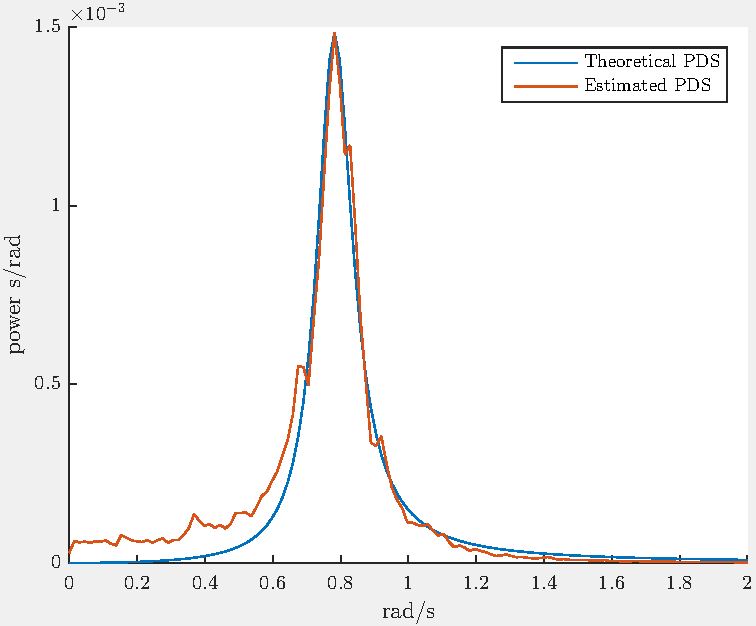
\includegraphics[width=0.5\textwidth]{images/2d-fitted_theoretical_PSD_vs_estimated_PSD}
    \caption{Fitted theoretical PSD vs estimated PSD}
    \label{fig:2d-fitted_theoretical_PSD_vs_estimated_PSD}
\end{figure}
